%% LyX 2.0.6 created this file.  For more info, see http://www.lyx.org/.
%% Do not edit unless you really know what you are doing.
\documentclass[english]{article}
\usepackage[T1]{fontenc}
\usepackage[latin9]{inputenc}
\usepackage{enumitem}
\usepackage{sidecap}
\usepackage{framed}
\usepackage{cprotect}
\usepackage{enumitem}
\usepackage{listings}
\usepackage{amstext}
\usepackage{amstext}
\usepackage{pdfpages}
\usepackage{alltt}
\usepackage{epstopdf}
\usepackage{xspace,colortbl}
\usepackage[USenglish]{babel}
\usepackage{multirow}
\usepackage{url}
\usepackage{subfigure}
\usepackage{graphicx}%%
\usepackage{amssymb}
\usepackage{fmtcount}
\usepackage{amsfonts}
\usepackage{xspace}
\usepackage{amsmath}
\usepackage{multirow}
\usepackage[mathscr]{eucal}
%\usepackage{psfrag}
\usepackage{colortbl}

\usepackage{bm}
\usepackage{times}
\usepackage[nospace]{cite}
\usepackage{csquotes}
\usepackage{enumitem}
\usepackage{geometry}
\geometry{verbose,tmargin=2.54cm,bmargin=2.54cm,lmargin=2.54cm,rmargin=2.54cm}
\usepackage{babel}
\begin{document}

\newtheorem{theorem}{Theorem}
\newtheorem{example}{Example}
\newtheorem{definition}{Definition}
\newtheorem{problem}{Problem}
\newtheorem{property}{Property}
\newtheorem{proposition}{Proposition}
\newtheorem{lemma}{Lemma}
\newtheorem{corollary}{Corollary}

\newcommand{\cond}{\textrm{pred}\xspace}
\newcommand{\dataset}{data set\xspace}
\newcommand{\datasets}{data sets\xspace}
\newcommand{\spview}{\textsf{SPView}\xspace}
\newcommand{\fjview}{\textsf{FJView}\xspace}
\newcommand{\aggview}{\textsf{AggView}\xspace}
\newcommand{\hashfunc}[1]{\textsf{hash}(#1)\xspace}
\newcommand{\hashop}{\textsf{hash}\xspace}
\newcommand{\nsc}{\textsf{NormalizedSC}\xspace}
\newcommand{\rsc}{\textsf{RawSC}\xspace}

\newcommand{\avgfunc}{\ensuremath{\texttt{avg} }\xspace}
\newcommand{\maxfunc}{\ensuremath{\texttt{max} }\xspace}
\newcommand{\minfunc}{\ensuremath{\texttt{min} }\xspace}
\newcommand{\histfunc}{\ensuremath{\texttt{histogram\_numeric} }\xspace}
\newcommand{\countfunc}{\ensuremath{\texttt{count}}\xspace}
\newcommand{\sumfunc}{\ensuremath{\texttt{sum} }\xspace}
\newcommand{\varfunc}{\ensuremath{\texttt{var} }\xspace}
\newcommand{\stdfunc}{\ensuremath{\texttt{std} }\xspace}
\newcommand{\covfunc}{\ensuremath{\texttt{cov} }\xspace}
\newcommand{\corrfunc}{\ensuremath{\texttt{corr} }\xspace}
\newcommand{\medfunc}{\ensuremath{\texttt{median} }\xspace}
\newcommand{\percfunc}{\ensuremath{\texttt{percentile} }\xspace}
\newcommand{\havingfunc}{\ensuremath{\texttt{HAVING} }\xspace}
\newcommand{\selectfunc}{\ensuremath{\texttt{select} }\xspace}
\newcommand{\ratio}{\ensuremath{\rho }\xspace}


\newcommand{\insertion}{\ensuremath{\texttt{INSERT} }\xspace}
\newcommand{\update}{\ensuremath{\texttt{UPDATE} }\xspace}
\newcommand{\delete}{\ensuremath{\texttt{DELETE} }\xspace}

\author{ Sanjay Krishnan, Jiannan Wang, Ken Goldberg, Michael J. Franklin \\
AMPLab, UC Berkeley\\
\{jnwang, sanjaykrishnan, franklin, goldberg\}@berkeley.edu
%\email{milo@cs.tau.ac.il,~~~~tim\_kraska@brown.edu}
}

\title{SampleClean: Fast and Reliable Analytics on Dirty Data}
\maketitle
\begin{abstract}
A perennial challenge in data analytics is presence of dirty data
in the form of missing, duplicate, incorrect or inconsistent values.
Data analysts report that data cleaning remains one of the most time
consuming steps in the analysis process, and data cleaning can require
a significant amount of developer effort in writing software or rules
to fix the corruption. Since \emph{a priori}, the magnitude of data
error is unknown, any amount of error is potentially biasing, and
this presents a dichotomy between facing the cost of data cleaning
or coping with consequences of unknown inaccuracy. In this article,
we present a line of work called SampleClean, which allows the analyst
to clean a sample of data and estimate the results (with provable
guarantees) of some types of analytics--building on results in Approximate
Query Process (AQP). We describe three projects: SampleClean, Stale
View Cleaning, and ActiveClean. SampleClean returns bounded estimates
of SUM, COUNT, and AVG queries using a sample of cleaned data. Stale
View Cleaning models staleness in Materialized Views as a type of
data error and applies and extenion of SampleClean for scalable incremental
maintenance. ActiveClean extends SampleClean to a class of analytics
that we call convex data analysis (subsuming common aggregate queries
and including Machine Learning). Finally, we describe a number of
open problems and future directions for the project.
\end{abstract}

\section{Introduction}
Data are susceptible to various forms of corruption such as missing,
incorrect, or inconsistent representations \cite{Gartner}.
Real-world data is commonly integrated from multiple sources, and the integration process may lead to a variety of data errors~\cite{DBLP:journals/pvldb/DongS13}. 
Data analysts report that data cleaning remains one of the most time
consuming steps in the analysis process \cite{nytimes}.
Identifying and fixing data error often requires manually inspecting data, which can quickly become costly and time-consuming. 
While crowdsourcing is an increasingly viable option for some types of errors ~\cite{DBLP:conf/sigmod/JefferyFH08,DBLP:journals/pvldb/FanLMTY10,DBLP:journals/pvldb/YakoutENOI11, gokhale2014corleone, park2014crowdfill, sampleclean,chu2015katara}, it comes at the significant cost of additional latency and the overhead of managing human workers. 

Ignoring the effects of dirty data is potentially dangerous.
Since \emph{a priori}, the magnitude of data error is unknown, any amount of error can be biasing.
Analysts have to choose between facing the cost of data cleaning
or coping with consequences of unknown inaccuracy.
In this article, we describe a middle ground that we call SampleClean \cite{wang1999sample, krishnan2015svc}; where an analyst can clean a sample of data, and use this sample to improve an erroneous query result.
The intriguing part of SampleClean is that while the query result is computed using a sample,                                   
results can often be more accurate than those computed over the full data due to the data cleaning.
This approximation error is boundable unlike the unknown data error, and the tightness of the bound is parametrized by a flexible cleaning cost (i.e., the sampling ratio).

The case for SampleClean is analogous to the case for Approximate Query Processing \cite{DBLP:conf/icde/OlkenR92, olken1993random, garofalakis2001approximate, AgarwalMPMMS13} (AQP).
For decision problems, exploratory analysis problems, and visualization, it often suffices to return an approximate query result bounded in confidence intervals; thus saving significant processing costs.
In many common aggregates, the samples-to-accuracy trade off tends to vary as $O(\frac{1}{\sqrt{n}})$, and therefore every additional $\epsilon$ factor of accuracy costs quadratically more. 
In applications where approximation can be tolerated, sampling avoids the expensive ``last mile" of processing and timely answers facilitate improved user experiences and faster analysis.

In traditional AQP, approximation necessarily sacrifices accuracy for reduced latency. 
However, the goal of SampleClean differs from AQP, as SampleClean trades off data transformation cost for gradual improvements in query accuracy through data cleaning.
While SampleClean introduces approximation error, the data cleaning mitigates errors in query results.
There is a break-even point where a sufficient amount of data is cleaned to facilitate an accurate approximation of queries on the cleaned data, and in this sense, sampling actually improves the accuracy of the query result.

SampleClean \cite{wang1999sample} and all of its extensions \cite{krishnan2015svc}, work in the \emph{budgeted data cleaning} setting. 
An analyst is allowed to apply an expensive data transformation $C(\cdot)$ to only $k\ll N$ rows in a relation.
One solution could be to draw $k$ records uniformly at random and apply data cleaning, e.g., a direct extension of AQP to the cleaned sample.
However, data cleaning presents a number of methodological problems that make this hard.
First, $C(\cdot)$ may change the sampling statistics, for example, duplicated records are more likely to be sampled.
Next, query processing on partially clean data, i.e., a mix of dirty and clean data, can lead to unreliable results due to the well known Simpsons Paradox.
Finally, high-dimensional analytics such as Machine Learning may be very sensitive to sample size, perhaps even more so than to dirty data, and techniques for avoiding sample size dependence are required.

One of the key insights is that there are two contrasting query processing techniques to address every budgeted data cleaning problem.
A direct extension of AQP can estimate the true query result based on the cleaned sample (possibly with some reweighting to account for changes in sampling statistics). 
A sample of cleaned data can also be used to correct the error in a query result over the dirty data.
There is an interesting theoretical tradeoff between these approaches, where the first approach is \emph{robust} as its accuracy is independent of the magnitude of data error, and the second approach is \emph{sample-efficient} as its accuracy is less dependent on sample size.

By establishing the link between AQP and data cleaning, this idea has opened up a number of new research opportunities. 
We applied the same principles to other domains with expensive data transformations such as Materialized View Maintenance and Machine Learning.
In this article, we highlight four projects:

\vspace{0.5em}
\noindent \textbf{\sampleclean \cite{wang1999sample}: } \sampleclean estimates aggregate (\sumfunc, \countfunc, \avgfunc) queries using samples of clean data. \sampleclean reweights the data to compensate for changes in sampling statistics such that the estimates are unbiased and bounded in confidence intervals.

\vspace{0.5em}
\noindent \textbf{View Cleaning \cite{krishnan2015svc}: } View Cleaning generalizes the notion of data cleaning to include expensive maintenance of out-of-date data. Staleness in materialized views (MVs) manifests itself as data error, i.e., a stale view has missing, superfluous, and incorrect rows.
Like data cleaning, eager MV maintenance is expensive, and View Cleaning models querying an MV as a budgeted data cleaning problem.
Aggregate queries are approximated from a stale MV using a small sample of up-to-date data, resulting in bounded estimates.

\vspace{0.5em}
\noindent \textbf{ActiveClean: } ActiveClean extends \sampleclean to a class of analytics problems called Convex Data Analytics (subsuming the aggregates studied in \sampleclean and including Machine Learning such as Support Vector Machines and Linear Regression). ActiveClean exploits the convex structure of the problem (i.e. gradients and feature space) to prioritize cleaning data that is likely to affect the model. ActiveClean directly integrates cleaning into the model training loop and as a result gives a bounded approximation for any cleaning budget.

\vspace{0.5em}
\noindent \textbf{Wisteria \cite{haas2015wisteria}: } Wisteria is a system that implements the ideas described in the SampleClean work in a distributed analytics platform. This involved designing an algebra for data cleaning transformations and optimizations for their execution to reduce the latency of data cleaning operators.

\vspace{0.5em}

This article is organized as follows. Section 2 introduces the project and its main ideas. Section 3 overviews the basic architecture of each one of the projects. Section 4/5/6 describes \sampleclean, View Cleaning, and ActiveClean respectively. Section 7 reviews the related work in this field. In Section 8, we highlight some of the open problems and future directions of the SampleClean project. Finally, we conclude in Section 9.
\section{Background and Main Ideas}

This section describes the key idea of SampleClean, namely, that data cleaning can be integrated with approximate query processing leading to bounded approximations of clean query results for a fraction of the cleaning cost.

\subsection{Data Cleaning is Often Expensive}
A number of surveys report that data cleaning is one of the most time consuming steps \cite{kandel2012enterprise, nytimes}.
Data cleaning frameworks have been recently proposed to address the problem of corrupted data at scale\cite{khayyat2015bigdansing, chu2015katara, sampleclean}.
As errors can be domain- or dataset-specific, data cleaning is an inherently human-driven process and can require a significant amount of developer effort in writing software or rules to fix the corruption.
Automated fixes may not be reliable and can require human confirmation \cite{DBLP:journals/pvldb/YakoutENOI11}.
One way to scale up human computation is crowdsourcing which has shown recent success in entity resolution and value filling \cite{gokhale2014corleone, park2014crowdfill, sampleclean,chu2015katara}.
However, crowdsourcing comes with the costs of significant additional latency (orders of magnitude slower than data processing) and the overhead of managing human workers.

\subsection{Traditional Approximate Query Processing}
The basic idea of AQP is to approximate the result of a query $Q$ on a large relation $R$, instead of processing the entire relation.
A number of approximation schemes have been proposed including using Sampling, Wavelets, Sketching, and Hashing (see Cormode et al. for a survey \cite{DBLP:journals/ftdb/CormodeGHJ12}).
This article focuses on Sampling-based approximations.
Sampling-based approximate query processing (SAQP) is a powerful technique that allows for fast approximate results on large datasets. 
It has been well studied in the database community since the 1990s~\cite{DBLP:conf/sigmod/HellersteinHW97,DBLP:conf/sigmod/AcharyaGPR99,DBLP:conf/icde/OlkenR92, OlkenR86}, and methods such as BlinkDB~\cite{DBLP:conf/eurosys/AgarwalMPMMS13} have drawn renewed attention in recent big data research. 
An important aspect of SAQP is confidence intervals, as many types of aggregates can be bounded with techniques such as concentration inequalities (e.g., Hoeffding bounds), large-deviation inequalities (e.g., Central Limit Theorem), or empirically (e.g., Bootstrap). 

Suppose, there is a relation $R$ and a uniform sample $S$.
SAQP applies a query $Q$ to $S$ (possibly with some scaling $c$) to return an estimate: 
\[
Q(R) \approx est = c \cdot Q(S)
\]

Traditionally, AQP sacrifices accuracy due to sampling for improved query latency.
However, bounds on $est$ assume that the only source of error is uncertainty introduced by sampling, however, the data itself may contain errors which could also affect query results.
When the data itself is erroneous, a query result on the full data--let alone a sample, will be incorrect.
The main argument for SampleClean is that when data errors significantly affect query results,
sampling can be combined with data cleaning to actually improve accuracy.
This leads to a counter-intuitive result where it is possible that a query on a cleaned sample of data is more accurate than a query on the entire dirty data.

\iffalse
\subsection{Exploiting Application Structure}

\jn{It's a little too early to present the content of this section before showing the big idea. I would suggest to put it either to the end of Sec 2 or the end of Sec 3. }

SampleClean applies sample to clean $k\ll N$ rows in a database to address the time-scale mismatch between the analytics application (e.g., SQL query, Machine Learning, Materialized View) and data cleaning.
An important aspect of this project is how the structure and semantics of that application can be used to prioritize and budget data cleaning.
A database only needs to be sufficiently clean for the requirements of the subsequent analytics--and the key insight from AQP being that aggregates are tolerant to approximation.

In the initial SampleClean work, we restricted the allowed aggregate queries to \sumfunc, \countfunc, and \avgfunc with predicates and group by clauses.
In the two subsequent projects, View Cleaning and ActiveClean, we expanded the scope and the semantics of the application. 
The View Cleaning problem explores data cleaning and general aggregates on derived relations with known view definitions.
We can exploit view definition to query just as much of the base data as needed to accurately answer the aggregate query for a fixed budget.
In fact, we showed that any aggregate (beyond \sumfunc, \countfunc, and \avgfunc) that could be estimated with SAQP\cite{agarwalknowing}, could be answered estimated with the View Cleaning framework.
ActiveClean generalizes the initial work on \sumfunc, \countfunc, and \avgfunc to higher-dimensional aggregates.
We defined a class of analytics called Convex Data Analytics, and show how the convex structure of the analytics can be used to guide and prioritize data cleaning.
\fi

\subsection{Approximate Query Processing on Dirty Data}


\subsubsection{Two Sources of Errors: Sampling Error and Data Error}
Now consider the case when the data is dirty.
If $R$ is dirty, then there is a true relation $R_{clean}$.
\[
Q(R_{clean}) \ne Q(R) \approx est = c \cdot Q(S)
\]
The error in $est$ has two components: error due to sampling $\epsilon_s$ and error due to the difference with the cleaned relation $\epsilon_c = Q(R_{clean}) - Q(R)$:
\[
\mid Q(R_{clean}) - est \mid \le \epsilon_s + \epsilon_c
\]

While they are both forms of query result error, $\epsilon_s$ and $\epsilon_c$ are very different quantities.
$\epsilon_s$ is a random variable due to the sampling, and different samples would result in different realizations of $\epsilon_s$.
As a random variable introduced by sampling, $\epsilon_s$ can be bounded by a variety of techniques as a function of the sample size.
On the other hand, $\epsilon_c$ is deterministic, and by definition is an unknown quantity until all the data is cleaned.
Thus, the bounds returned by a typical AQP framework on dirty data would neglect $\epsilon_c$.

It is possible that $R_{clean} \ne R$ but $\epsilon_c=0$.
Consider a \sumfunc query on the relation $R(a)$, where $a$ is a numerical attribute.
If half of the rows in $R$ is corrupted with $+1$ and the other half are corrupted with $-1$, then $Q(R_{clean}) = Q(R)$.
The interesting problem is when there are \emph{systematic errors}\cite{taylor1982introduction} i.e., $\epsilon_c > 0$. 
In other words, the corruption that is correlated with the data, e.g., where every record is corrupted with a $+1$.

\subsubsection{Key Idea I: Direct Estimate vs. Correction}
The key quantity of interest in this work is $\epsilon_c$, and to be able to bound
a query result on dirty data, requires that $\epsilon_c$ is 0 or bound $\epsilon_c$.
There are two ways in which this can be done: direct estimates and corrections.

\vspace{0.5em}
\noindent\textbf{Direct Estimate (Figure \ref{fig:est}A): } This technique is a direct extension of SAQP to handle data cleaning. A set of $k$ rows is sampled uniformly at random from the dirty relation $R$ resulting in a sample $S$. Data cleaning is applied to the sample $S$ resulting in $S_{clean}$.
Data cleaning and sampling may change the statistical and scaling properties of the query $Q$, so $Q$ may have to be re-written to a query $\widehat{Q}$. $\widehat{Q}$ is applied to the sample $S_{clean}$ and the result is returned. 
There are a couple of important points to note about this techniques.
First, as in SAQP, the direct estimate only processes a sample of data.
Next, since it processes a cleaned sample of data, at no point is there a dependence on the dirty data.
As we will show later in the article, the direct estimate returns a result whose accuracy is independent of the magnitude or rate of data error. 
From a theoretical perspective, for some types of data cleaning, this technique ensures that $\epsilon_c = 0$ within the sample.

\vspace{0.5em}
\noindent\textbf{Correction (Figure \ref{fig:est}B): } The direct estimate suffers a subtle drawback. Suppose, there are relatively few errors in the data. The errors introduced by sampling may dominate any error reductions due to data cleaning. Instead of the direct estimate which ensures $\epsilon_c = 0$, we can try to estimate $\epsilon_c$. A set of $k$ rows is sampled uniformly at random from the dirty relation $R$ resulting in a sample $S$. Data cleaning is applied to the sample $S$ resulting in $S_{clean}$. 
The difference in applying $\widehat{Q}$ to S and $\widehat{Q}$ to $S_{clean}$ gives an estimate of $\epsilon_c$. 
The interpretation of this estimate is a correction to the query result on the full dirty data.
In contrast to the direct estimate, this technique requires processing the entire dirty data (but only cleaning a sample).
However, as we will later show, if errors are rare this technique gives significantly improved accuracy over the direct estimates.

\begin{SCfigure}\centering
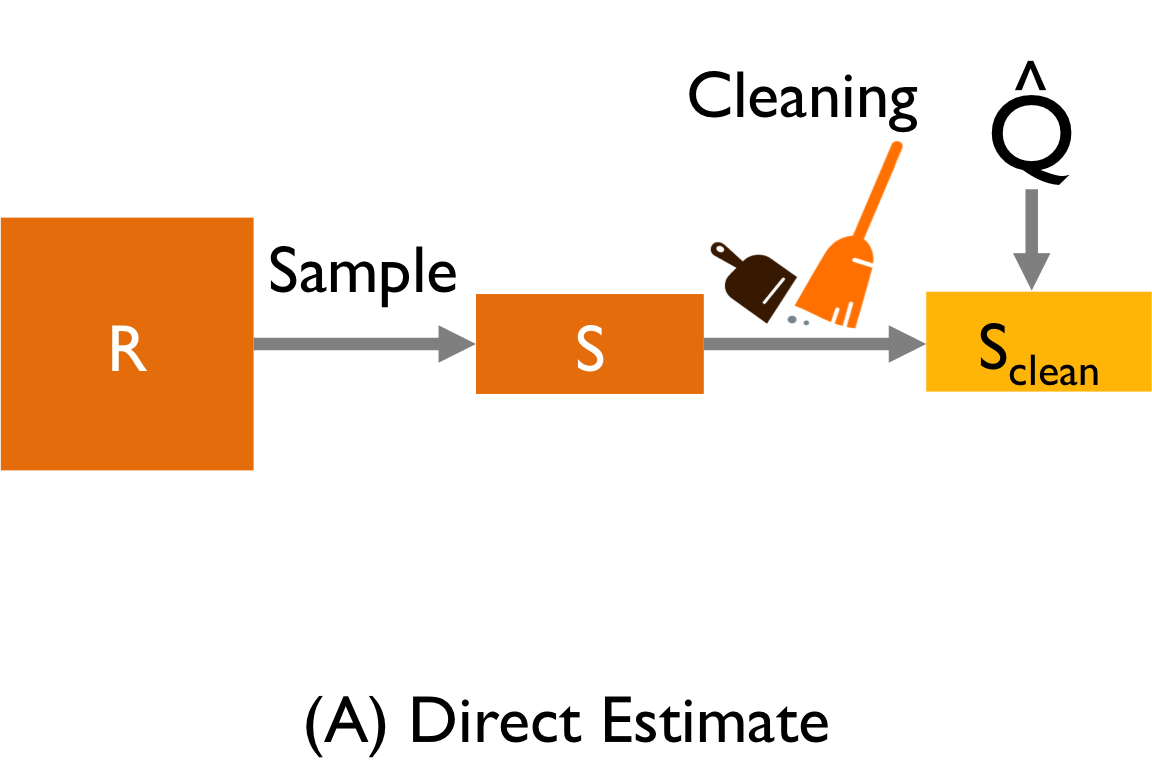
\includegraphics[width=.3\columnwidth]{figs/est1b.png}
\hspace{2em}
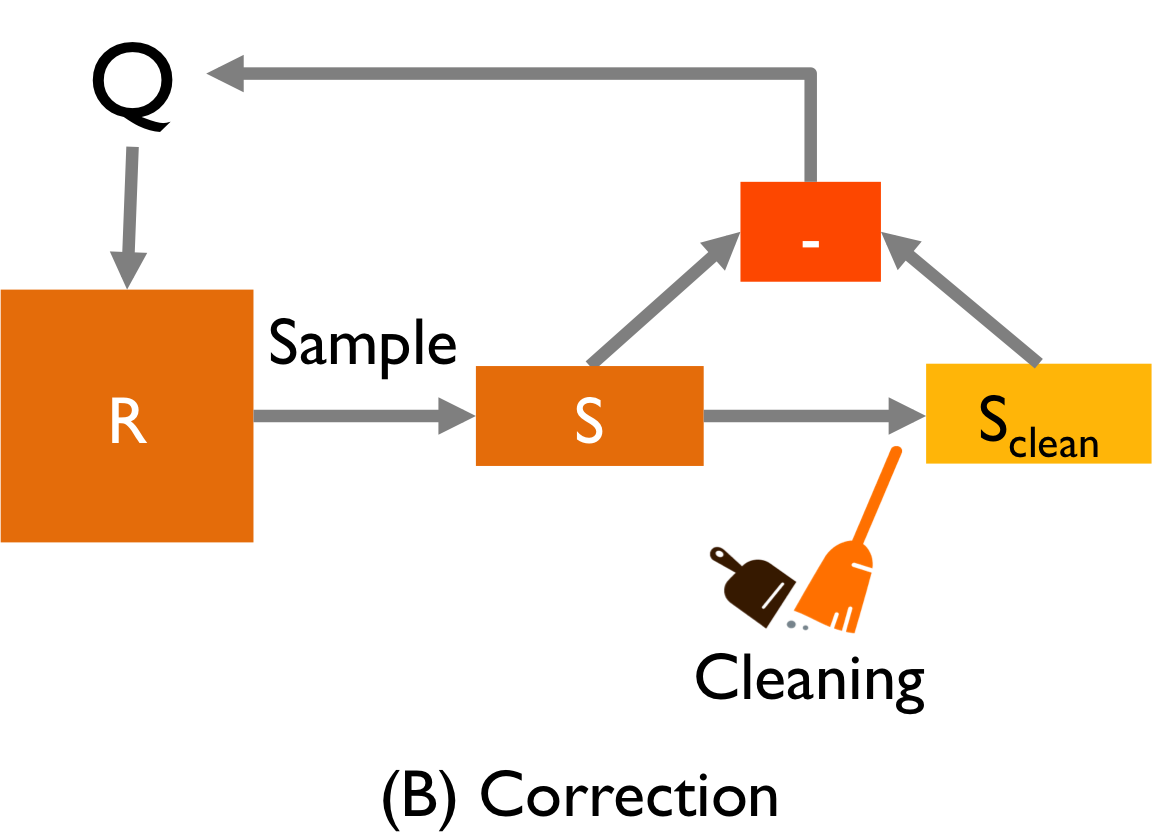
\includegraphics[width=.3\columnwidth]{figs/est1c.png}
\caption{Estimating query results with data cleaning on random samples. There are two ways to estimate a query result: (a) direct estimation applies the query to a sample (possibly with some scaling), and (b) correction corrects a query result on the entire dirty data.\label{fig:est}}
\end{SCfigure}

\subsubsection{Key Idea II: Sampling to Improve Accuracy}
A small sample of clean data can improve improve query accuracy accuracy.
Figure \ref{fig:est2} plots error as a function of the cleaned sample size on a corrupted TPCH dataset for a direct estimate, correction, and AllDirty (query on the full dirty data).
In both cases, there is a break-even point (in terms of number of cleaned samples) when the data cleaning has mitigated more data error than the approximation error introduced by sampling.
After this point, SampleClean improves query accuracy in comparison to AllDirty.
When errors are relatively rare (5\% corruption rate), the correction is more accurate. 
When errors are more significant (50\% corruption rate), the direct estimate is more accurate.
Note that the direct estimate returns results of the same accuracy regardless of the corruption rate. 

\begin{SCfigure}
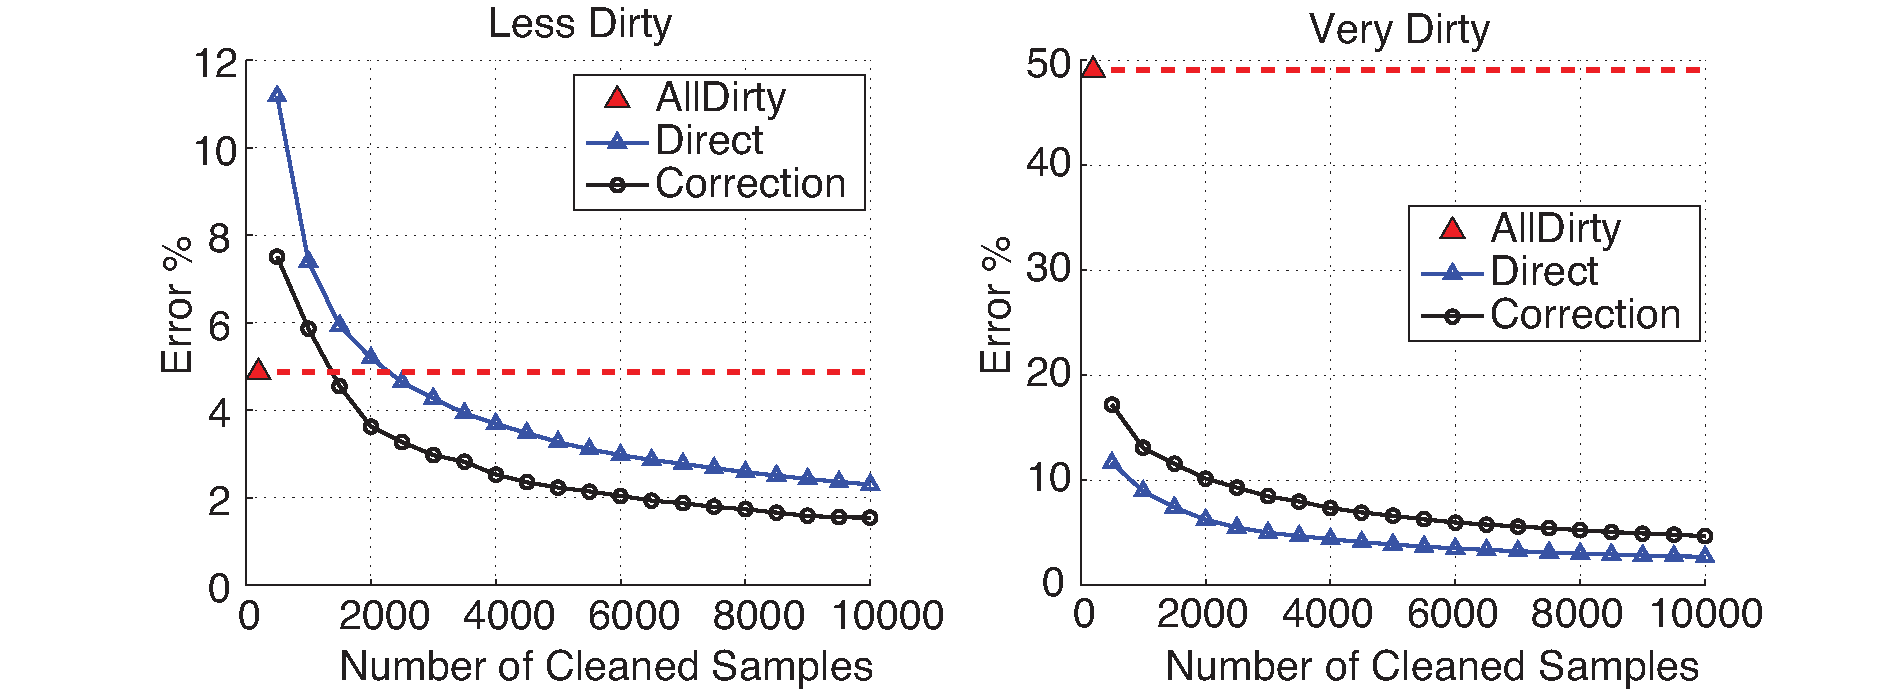
\includegraphics[width=.6\columnwidth]{figs/allerror-samplesize.pdf}
\caption{Comparison of the convergence of the methods on two TPC-H datasets of 6M tuples with simulated errors 50\% error and 5\% error. On the dataset with larger errors, the direct estimate gives a narrower confidence interval, and on the other the correction is more accurate. \label{fig:est2}}
\end{SCfigure}





\fontsize{8.4pt}{8.7pt} \selectfont
\bibliographystyle{abbrv}
\bibliography{ref} 

\end{document}

